%%%%%%%%%%%%%%%%%%%%%%%%%%%%%%%%%%%%%%%%%%%%%%%%%%%%%%%%%%%%%%%%%%%%%%%% 
%%%%%%%%%%%%%%%%%%%%%%%%%%%%%%%%%%%%%%%%%%%%%%%%%%%%%%%%%%%%%%%%%%%%%%%% 
\begin{frame}[fragile=singleslide]
  \frametitle{Hands-On 4 : Finite Difference / Stencil}

  \hypertarget{handson4}{}

  \begin{itemize}
  \item Purpose:
    \begin{itemize}
    \item Illustrate the use of 2D/3D \texttt{Kokkos::View}
    \item Illustrate the use of alternative execution policies: \texttt{Kokkos::Experimental::MDRangePolicy}, \texttt{Kokkos::TeamPolicy},...
    \end{itemize}
  \item Stencil kernel:
    \begin{minted}[autogobble,obeytabs=true,tabsize=2]{c++}
      for (int k=0; k<nz; ++k)
        for (int j=0; j<ny; ++j)
          for (int i=0; i<nx; ++i) {
            y(i,j,k) = -5*x(i,j,k) +
              ( x(i-1,j  ,k  ) + x(i+1,j  ,k  ) +
                x(i  ,j-1,k  ) + x(i  ,j+1,k  ) +
                x(i  ,j  ,k-1) + x(i  ,j  ,k+1) );
          }
    \end{minted}
  \item exercise located in \url{code/handson/4/stencil}
  \end{itemize}
  
\end{frame}

%%%%%%%%%%%%%%%%%%%%%%%%%%%%%%%%%%%%%%%%%%%%%%%%%%%%%%%%%%%%%%%%%%%%%%%% 
%%%%%%%%%%%%%%%%%%%%%%%%%%%%%%%%%%%%%%%%%%%%%%%%%%%%%%%%%%%%%%%%%%%%%%%% 
\begin{frame}[fragile=singleslide]
  \frametitle{Hands-On 4 : Finite Difference / Stencil}

  Work to do:
  \begin{itemize}
  \item follow \texttt{readme}
  \item Once the kernels are done, you compare the performance
    \begin{itemize}
    \item the difference between kernel implementations, for different sizes
    \item CPU / GPU
    \end{itemize}
  \end{itemize}
  
\end{frame}

%%%%%%%%%%%%%%%%%%%%%%%%%%%%%%%%%%%%%%%%%%%%%%%%%%%%%%%%%%%%%%%%%%%%%%%% 
%%%%%%%%%%%%%%%%%%%%%%%%%%%%%%%%%%%%%%%%%%%%%%%%%%%%%%%%%%%%%%%%%%%%%%%% 
\begin{frame}
  \frametitle{Hands-On 4 : Finite Difference / Stencil}

  Example of performance obtained on different architectures (can be reproduced using \url{https://github.com/pkestene/kokkos-proj-tmpl/}):

  \begin{itemize}
    \only<1>{
    \item On Intel skylake (1 socket, 24 cores)\\
      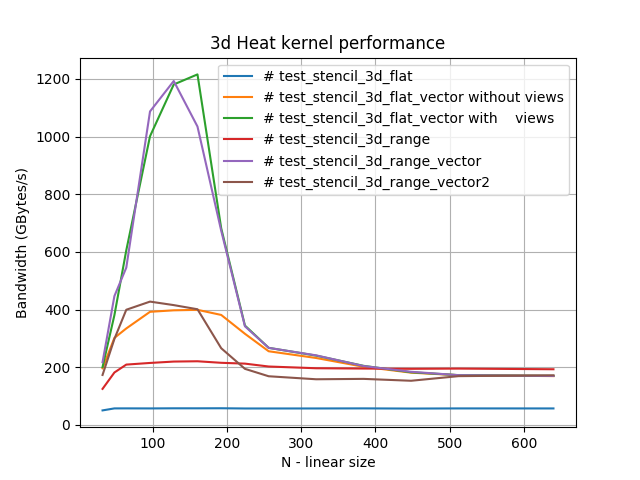
\includegraphics[width=7.5cm]{images/stencil/plot_stencil_perf_irene_skx}
    }
    \only<2>{
    \item On Nvidia K80\\
      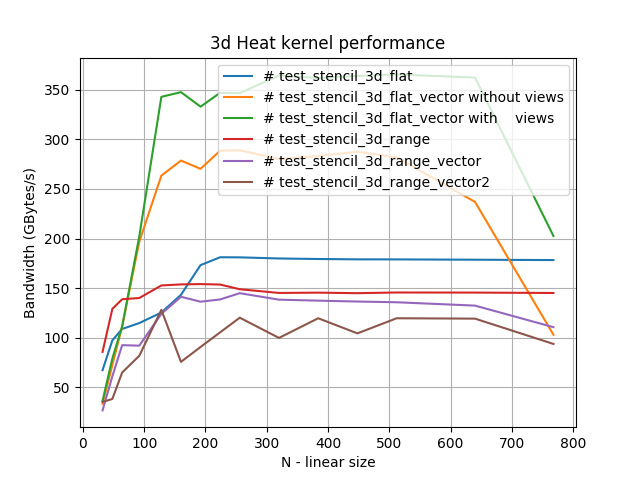
\includegraphics[width=7.5cm]{images/stencil/plot_stencil_perf_k80}
    }
    \only<3>{
    \item On Nvidia P100\\
      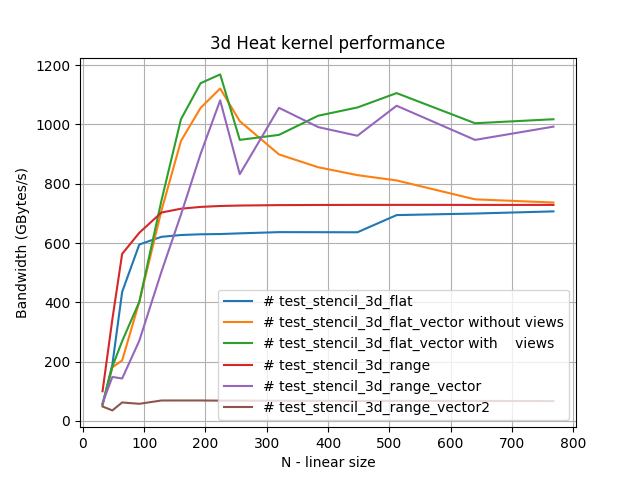
\includegraphics[width=7.5cm]{images/stencil/plot_stencil_perf_p100}
    }
  \end{itemize}
  
\end{frame}